\documentclass{report}
\usepackage[utf8]{inputenc}
\usepackage{graphicx}
\usepackage{geometry}
\geometry{top=10pt}

\usepackage{titlesec}
\usepackage{lipsum}
\titleformat{\chapter}[display]
 {\normalfont\bfseries}{}{0pt}{\LARGE} 


\title{PROJECT PLAN - ERB TELEMETRY}
\author{Simone Manenti 1048788\\ Cattaneo Federico 1053265}



\begin{document}

\maketitle

\chapter{INTRODUZIONE}
\subsection{Storia}
Durante la fase di progettazione svolta dal gruppo di controllo del team ERB di Formula SAE, dell'Università degli Studi di Bergamo, si è scoperta la necessità di dover leggere i dati dei sensori collegati alla centralina, visualizzarli a schermo per poter fare un'analisi in tempo reale e verificare che nel sistema tutti i sensori siano in uno stato accettabile.
Non trovando un software gratuito che andasse incontro alle esigenze del team, abbiamo deciso di sviluppare un software con le funzionalità essenziali per poter far procedere il team con la fase di test.
\\
Le necessità del team sono di visualizzare a schermo i dati in tempo reale, tramite tabelle o tramite grafici (funzionalità opzionale) e di salvare questi dati su file, per poter eventualmente confrontare i dati di due sessioni di test e capire se, a seguito di modifiche alla vettura, queste siano efficaci oppure siano modifiche non necessarie o controproducenti.


\chapter{Descrizione del progetto}
Nel sistema sono presenti due Arduino:
\begin{itemize}
\item \textbf{Arduino TX}: collegato alla centralina, si occupa della trasmissione dei dati dalla vettura ad un ricevitore.
\item \textbf{Arduino RX}: collegato ad un computer, si occupa della ricezione dei dati inviati dall'arduinoTX e all'inoltro degli stessi verso il PC tramite USB.
\end{itemize}

\subsection{Funzionalità}

\begin{itemize}
\item Riceviamo i dati in real time dei sensori collegati alla centralina nel formato: "acceleratore, pressione freno, temperatura freno, temperatura batteria, carica batteria, tempo sul giro, pressione gomme".
\item I dati possono essere visualizzati in real time tramite tabelle o grafici.
\item I dati possono essere salvati in un database locale .
\item Possiamo accedere allo storico dei dati salvati nel database locale.
\item L'utente che è autorizzato, può eliminare i dati non necessari, presenti nel database locale.
\end{itemize}


\subsection{Utenti}
Ci sono due possibili Livelli utente, “CapoReparto” e “IngegnereDiPista”.\\

L'IngegnereDiPista può:\\
\begin{itemize}
\item Accedere ai dati della telemetria e visualizzarli a schermo tramite grafici o tabelle.
\item Selezionare quali tipi di dati sono da visulizzare.
\item Selezionare l’intervallo di tempo dei dati che vuole visualizzare.\\
\end{itemize}

Il CapoReparto può:
\begin{itemize}
\item Svolgere tutte le funzioni dell’IngegnereDiPista.
\item Selezionare dei dati ed eliminarli dal database locale.
\end{itemize}

\subsection{Comportamento comunicazione real time}
\begin{itemize}
\item La monoposto trasmette i dati in modalità broadcast a prescindere dalla presenza di ricevitori collegati.
\item Qualsiasi utente, tramite pulsante, decide quando avviare la comunicazione con il ricevitore.
Se la comunicazione è avvenuta, i dati possono essere visualizzati tramite tabella e contemporaneamente salvati in locale.
\item L’utente può interrompere la comunicazione a piacimento (implica lo stop della lettura e scrittura dei dati).
\item Se la connessione tra il PC e il ricevitore non avviene, deve apparire un messaggio di errore.
\end{itemize}

\subsection{Comportamento dati in locale}
\begin{itemize}
\item Qualsiasi utente può visualizzare i dati salvati nel database locale tramite tabelle o grafici.
\item Qualsiasi utente può esportare i grafici o le tabelle.
\item L’utente CapoReparto può selezionare ed eliminare i dati presenti nel Database.
\end{itemize}





\chapter{MODELLO DI PROCESSO}
Abbiamo deciso di adottare un modello di processo Agile ibrido per i seguenti motivi:
\begin{itemize}
\item Il team ERB attualmente non ha una visione completa del sistema
\item Vogliamo procedere a piccoli incrementi per poter avere una qualità maggiore 
\item Potrebbero avvenire cambiamenti dell'interfaccia e delle funzioni
\item Dobbiamo ottimizzare il tempo a disposizione per lo sviluppo del sistema
\end{itemize}

\subsection*{Must have:}
\begin{itemize}
\item Gestione porta COM comunicazione con ricevitore
\item Gestione database locale per archiviazione/consultazione storico dati.
\item GUI: Visualizzazione real-time dei dati ricevuti.
\item GUI: Gestione porta COM 
\item GUI: Visualizzazione tabellare storico dati
\item GUI: Grafico dei trend 
\item GUI: Visualizzazione errori di connessione
\item Export dello storico dati tramite file CSV
\end{itemize}

\subsection*{Requisiti Should have:}
\begin{itemize}
\item GUI: identificazione tramite colore dei valori che richiedono l'attenzione dell'operatore
\item Accesso utenti
\end{itemize}

\subsection*{Could have:}
\begin{itemize}
\item Possibilità di muovere i componenti grafici all'interno dell'interfaccia
\item Possibilità di cambiare il tema dell'interfaccia
\end{itemize}

\subsection*{Would have:}
\begin{itemize}
\item Possibilità di inviare comandi alla monoposto
\end{itemize}


\chapter{ORGANIZZAZIONE DEL PROGETTO}
Avendo deciso di usare un modello SCRUM, ci troviamo a dover assegnare ognuno dei tre ruoli ad entrambi i membri del Team.\\
I ruoli di SCRUM Master, Product owner e Development Team saranno ricoperti da:
\begin{itemize}
\item Cattaneo Federico
\item Simone Manenti
\end{itemize}
Entrambi i membri del Team hanno pari responsabilità all'interno del progetto.

\begingroup
\let\clearpage\relax
\chapter{STANDARD. LINEE GUIDA E PROCEDURE}
\endgroup

Le procedure che il team dovrà seguire sono:
\begin{itemize}
\item Individuazione dei requisiti, stima dei costi e delle tempistiche
\item Progettazione dei modelli UML su cui si baserà il codice
\item Implementazione del codice
\item Verifica della qualità e della validità
\end{itemize}
Per la gestione delle versioni del sistema utilizziamo GIT, per alcune componenti useremo uno sviluppo simile a quello adottato nell'extreme programming, nel quale entrambi i membri del Team programmeranno sulla stessa macchina.\\
Gestiamo la priorità dei requisiti secondo le regole MoSCoW\\
Adotteremo le linee guida ISO/IEC 9126


\chapter{ATTIVITÀ DI GESTIONE}
Dopo esserci occupati dell'individuazione dei requisiti e aver fatto la prima stesura del Product Backlog, dobbiamo occuparci dello Sprint Planning.	\\
\textbf{Sprint:}\\
\begin{itemize}
\item La durata di ogni sprint sarà di 7 giorni.
\item Al termine del primo Sprint avverrà il rilascio di una prima versione del software, che non conterrà tutti i requisiti individuati nel Product Backlog, ma fungerà da Prototipo.
\item Al termine del secondo Sprint, verrà rilasciata una versione software contenente tutti i requisiti "Must Have".
\item Nei successivi Sprint andremo ad implementare i requisiti "Should have" ed eventuali nuovi requisiti "Must Have" e ci concentreremo principalmente sul miglioramento degli elementi già implementati nel software.
\item Al termine di ogni Sprint presentiamo il software al team ERB per avere un feedback utile per apportare modifiche o individuare nuove funzionalità.
\end{itemize}

\textbf{Daily scrum:}\\
\begin{itemize}
\item I membri del team, a fine giornata, si riuniranno per pianificare l'attività del giorno dopo.
\end{itemize}


\chapter{RISCHI}
Abbiamo individuato diverse tipologie di rischi:
\begin{itemize}
\item Ritardo nel rappresentare i dati ricevuti dal trasmettitore
\item Possibilità di ottenere grafici non intuitivi da leggere
\item Errore di eliminazione dei dati sul database da parte del Capo Reparto
\item Possibilità di perdita dei dati nel caso in cui ci sia un guasto dell'hardware, poiché il database è locale, sulla macchina dell'utente
\end{itemize}

\begingroup
\let\clearpage\relax
\chapter{PERSONALE}
\endgroup
Entrambi i membri del team:
\begin{itemize}
\item Entrambi i membri del team avranno pari responsabilità e si divideranno equamente le attività da svolgere.
\item Partecipano, gratuitamente, dalle prime fasi del progetto.
\item Hanno dovuto imparare ad utilizzare i vari software e tools proposti per lo sviluppo del sistema, ad esempio:
 Maven, StarUML, GitHub.
\item Hanno conoscenze di base del linguaggio Java.
\item Non hanno competenze sulla libreria SQLite.
\end{itemize}

\chapter{METODI E TECNICHE}
Per lo sviluppo del progetto utilizziamo diversi software e tools:
\begin{itemize}
\item Eclipse e Maven
\item SQLite
\item GitHub
\item StarUML
\item SceneBuilder e Javafx
\item Texmaker
\end{itemize}
Per gestire la configurazione e tener traccia delle modifiche apportate al software, utilizziamo la notazione orientata alla versione;\\
Ogni modifica genererà una versione numerata del software (ad esempio: X.0.1).

\chapter{GARANZIA DI QUALITÀ}
Il progetto è basato sul modello ISO 9126.\\
Durante la progettazione e l'implementazione, il team cerca di rispettare le caratteristiche di Funzionalità, Affidabilità, Usabilità, Efficienza, Manutenibilità e Portabilità che sono definite nel modello di qualità interno, cioè del codice sorgente, e nel modello esterno, cioè la qualità quando il software viene eseguito, dell'ISO.\\
Utilizzando il modello ISO 9126 il team ERB è interessato alla qualità in uso, cioè quando il team eseguirà il software durante le fasi di test dell'autovettura.\\
Per andare in contro a questo dovremo coordinare in modo adeguato la fase di progettazione e implementazione, utilizzando un ciclo di vita adeguato per poter soddisfare tutti i requisiti.\\
Dovremo anche sviluppare dei casi di test mirati, per simulare l'ambiente nel quale verrà eseguito il software.


\chapter{PACCHETTI DI LAVORO}
Dobbiamo suddividere il lavoro in diverse attività, alle quali entrambi i membri parteciperanno.\\
Organizziamo il lavoro tramite l'utilizzo della seguente WBS (work breakdown structure):

\begin{figure}[hbt!]
  \noindent\makebox[\textwidth]{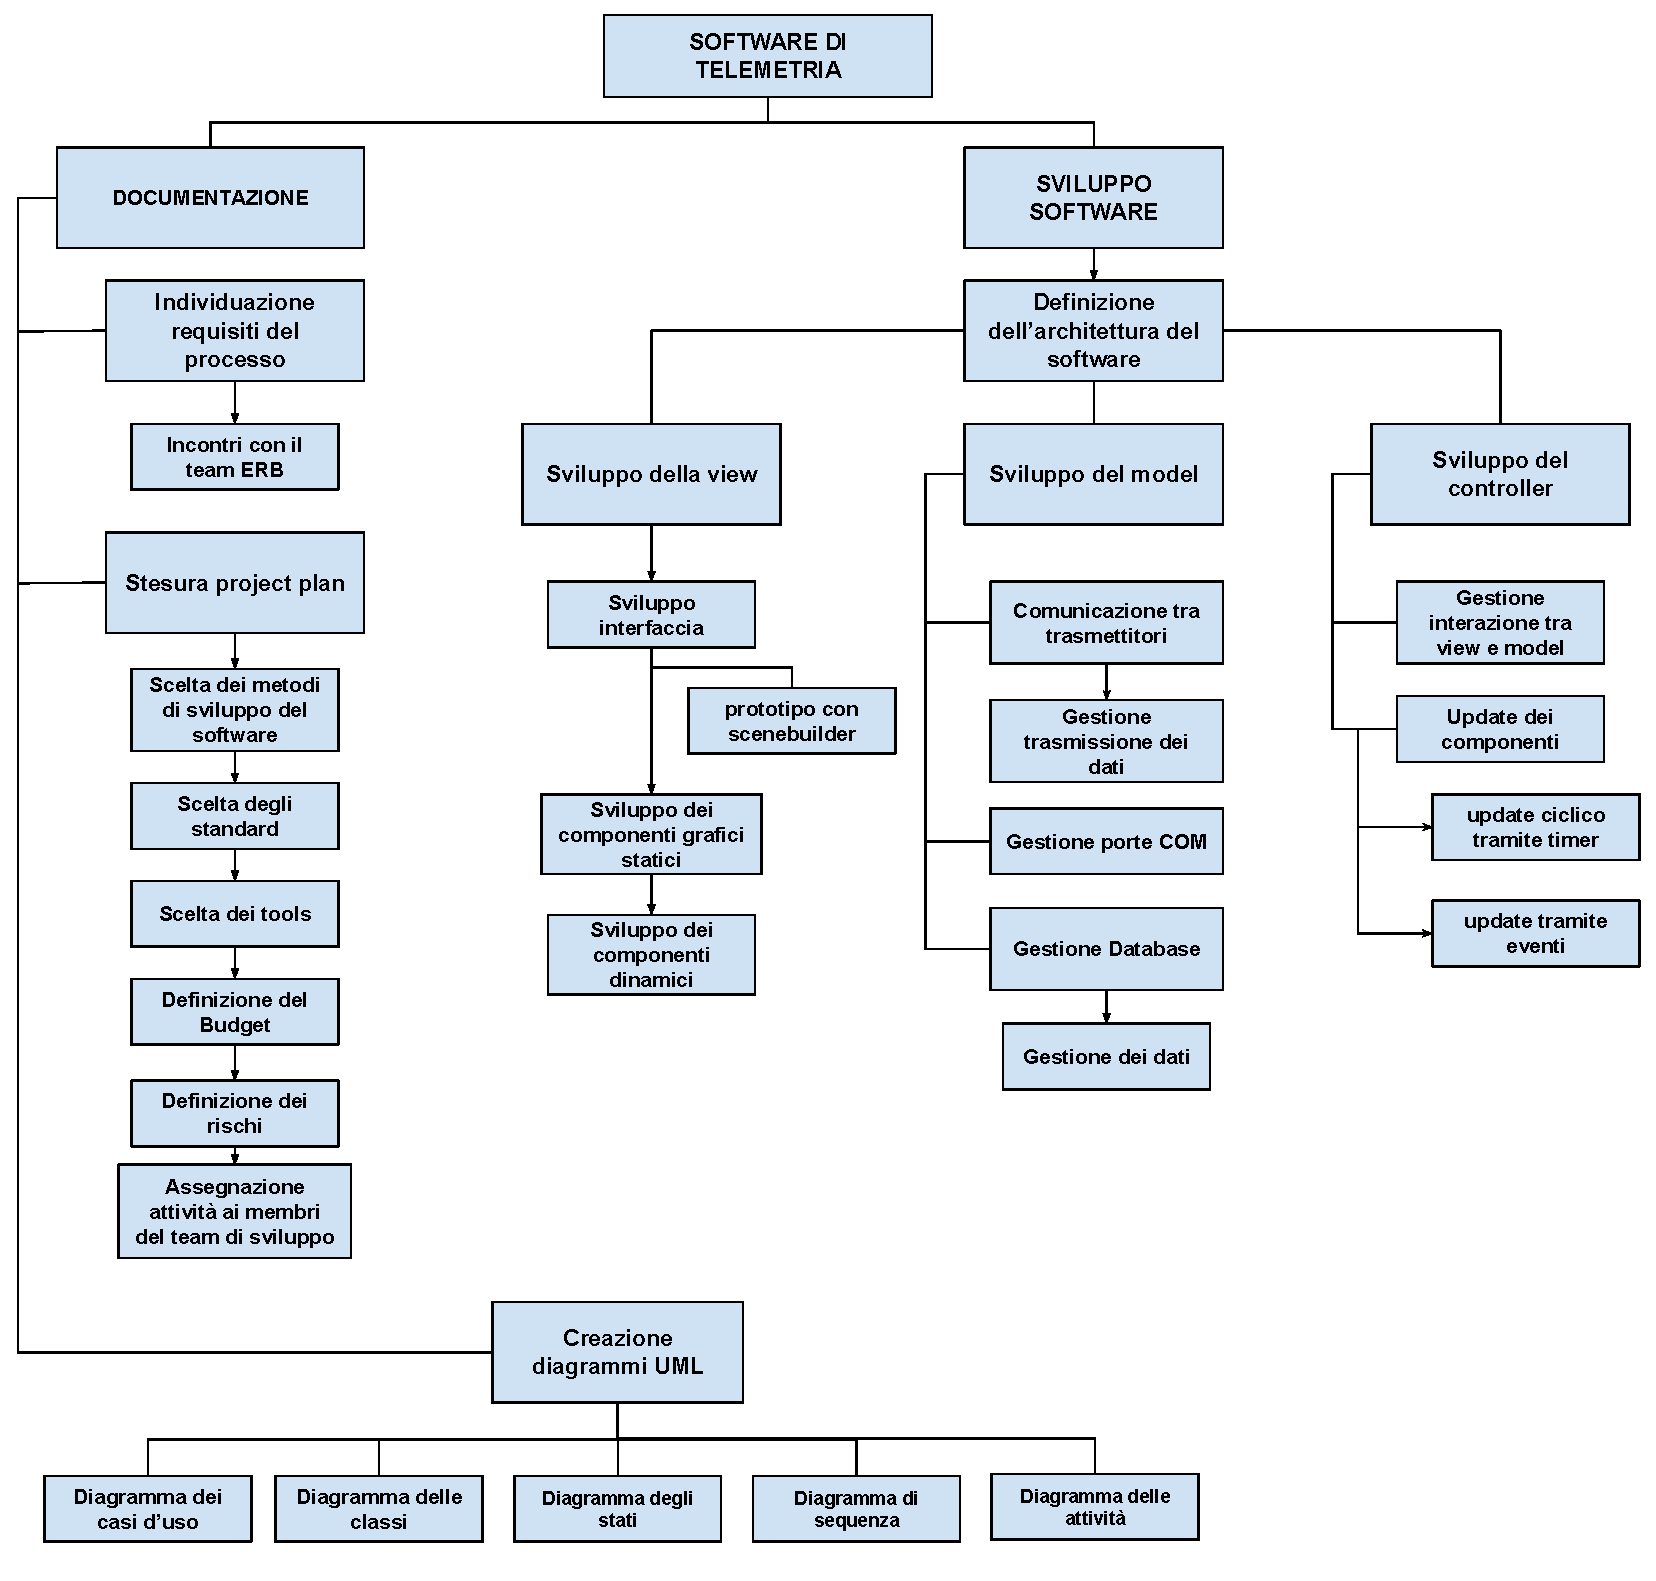
\includegraphics[width=1.4\textwidth]{wbs.pdf}}
\end{figure}

%
%In ordine dovremo fare le seguenti attività:
%\subsection*{Comunicazione con il cliente e requisiti del sistema}
%Fare degli incontri con il team ERB dell'Università degli Studi di Bergamo per poter definire i requisiti del progetto
%\subsection{Scelta ciclo di vita del progetto}
%Decidere come organizzare il lavoro
%\subsection*{Creazione grafici UML}
%Dedicare una parte del tempo per creare i diagrammi UML, in particolare i diagrammi degli stati, per poter creare una struttura di partenza per il software.
%\subsection*{Software:}
%Dividiamo l'attività di creazione del software in diverse sotto-attività:
%\subsubsection{Scelta dei tool}
%Fare degli incontri per scegliere i tool da utilizzare per la creazione dell'interfaccia grafica e per la creazione del database.
%\subsubsection{Creazione interfaccia grafica}
%Fare degli incontri per trovare la soluzione migliore per la scelta della composizione dell'interfaccia grafica e successivamente presentarla al team.
%\subsubsection{Interazione con interfaccia grafica}
%Implementare l'interazione con l'interfaccia grafica, le componenti dinamiche come pulsanti, gauge graphs e dropdown.
%\subsubsection{Creazione database}
%Implementare il database per la gestione dei dati
%\subsubsection{Comunicazione tra gli arduino}
%Implementare la comunicazione tra i dispositivi 
%\subsubsection{Implementazione elementi dinamici del programma}
%Implementare gli elementi grafici dinamici, come i grafici lineari che si aggiornano tramite i dati in real time\\\\
%\textbf{Documenti:} Abbiamo documentato tutte le attività nel documento denominato \textbf{Sprint}, presente nella sezione "Documenti" 

\chapter{RISORSE}
Le funzioni svolte dal software non richiedono grandi quantità di potenza computazionale e generalmente non richiedono grandi quantità di memoria per il salvataggio dei dati.\\

\begingroup
\let\clearpage\relax
\chapter{BUDGET}
\endgroup

Il progetto è diviso in Milestone:
\textbf{Inizio del progetto:} 
\begin{itemize}
\item L'obiettivo è di individuare il problema da risolvere, i requisiti per risolverlo e descrivere gli obiettivi.
\item Concluso in data 16/12/2023
\end{itemize}

\textbf{Stesura Project Plan:}
\begin{itemize}
\item L'obiettivo è quello di generare il project plan
\item Concluso in data 26/12/2023
\end{itemize}

\textbf{Elaborazione dei modelli UML:}
\begin{itemize}
\item L'obiettivo è quello di ottenere l'architettura del software tramite diagrammi UML
\item Concluso in data 29/12/2023
\end{itemize}

\textbf{Generazione del codice:}
\begin{itemize}
\item L'obiettivo è quello di generare il codice a partire dai modelli UML ottenuti nella Milestone precedente ed avere le prime versioni preliminari del software
\item Da concludere entro 01/01/2024
\end{itemize}

\textbf{Conclusione del progetto:}
\begin{itemize}
\item L'obiettivo è quello di verificare e validare il software e consegnare la versione definitiva al team ERB, per poterlo presentare durante la presentazione del progetto del team ERB agli eventuali sponsor.
\item Da concludere entro 09/02/2024
\end{itemize}

\chapter{CAMBIAMENTI}
Al termine di ogni Sprint, se vengono proposti dei cambiamenti da parte del team ERB, verranno inseriti all'interno del Product Backlog per poter procedere con lo Sprint planning.\\
Verranno anche aggiornati i documenti e verranno rilasciate le versioni del software con la numerazione descritta precedentemente.

\begingroup
\let\clearpage\relax
\chapter{CONSEGNA}
\endgroup

Al termine di ogni sprint, nel caso in cui siano state sviluppate nuove versioni del software, verrà consegnata al team ERB la versione più recente e verranno descritte le funzionalità aggiunte.\\
Ad ogni versione consegnata al team ERB, verrà rilasciata anche la documentazione inerente per poter facilitare l'utilizzo del software.\\\\
La versione finale del software verrà rilasciata solo dopo la fase di validazione e verifica fatta quando tutti i requisiti presenti nella categoria "Must Have" sono presenti all'interno del software.


\end{document}